\section{Forking and Its Empirical Structure}
\label{sec:empirical}

\subsection{Setting and phenomenon}
\label{sec:setting}

We use a NanoGPT backbone with 8 layers, 6 attention heads, a hidden dimension of 768, a vocabulary of 8192 tokens, and a sequence length of 2048, together with separate bigram and trigram lookup tables. Retrieved embeddings are injected at one of three routes---token representations before attention (input), attention values ($v$), or attention output ($y$)---alongside a no-gram baseline (Figure~\ref{fig:injection-routes}); the input route is the default. The backbone uses AdamW with learning rate $6\times10^{-4}$; the tables use momentum-free RMSProp at $128$ times the backbone learning rate. Learning rates are warmed up for 100 steps and then held constant. One epoch over the fixed single-shard training corpus takes 337 steps, and runs use seed 42 unless stated otherwise. Appendix~\ref{app:setting} gives the full contract, numerical precision, and implementation details.

Training loss ($L_{\mathrm{tr}}$) is the mean next-token cross-entropy on the current training batch, computed before the parameter update. Validation loss ($L_{\mathrm{va}}$) is the mean next-token cross-entropy on fixed held-out validation batches, evaluated after the update. At each evaluation step, the online gap is $G=L_{\mathrm{va}}-L_{\mathrm{tr}}$.

Figure~\ref{fig:injection-curves} shows the signature pattern over 2000 updates, with dotted lines marking the 337-step replay boundaries. During the first epoch, training and validation losses improve together. Once the same text is replayed, training loss keeps falling without a corresponding validation improvement, and the gap widens---not smoothly but in a staircase aligned with the replay boundaries: most of the damage arrives right after each epoch transition and accumulates over successive passes. All three over-encoding routes fork; the attention routes ($v$, $y$) fork far more strongly than the input route, while the no-gram baseline stays small. The phenomenon is not specific to this minimal architecture: a 12-layer DeepSeek-style model with multi-layer Engram input over-encoding reproduces forking and responds to low-frequency read masking in the same way (Appendix~\ref{app:deepseek}).

\subsection{Empirical scaling laws}
\label{sec:forking-factors}

All experiments below use input injection, seed 42, and, where tables are enabled, a table learning rate $128$ times the backbone learning rate. The frequency analysis uses fixed probe losses on both sides; the remaining experiments use the online gap of Section~\ref{sec:setting}.

\paragraph{Context frequency.}
A finite corpus does not fully represent the continuation distribution of each context: a context whose population distribution assigns equal probability to $C$ and $D$ may appear three times with $C$ and once with $D$ in training, so fitting the sample underpredicts $D$ on fresh data. Enabling both tables ($2^{20}$ rows each) and measuring context-matched fixed-probe gaps at step 1000, grouped by the context count $F$ in the unrepeated corpus, shows that low-frequency contexts have systematically larger gaps, approximately as a power law in $F$ over the measured range (Figure~\ref{fig:frequency}; markers are token-mass-weighted bin means with within-bin standard deviations, dashed lines the fits derived in Section~\ref{sec:coverage}).

\paragraph{Table capacity.}
Bigger tables make forking worse. Across three decades of table rows $R$ in bigram-only and trigram-only models, the step-1000 gap generally increases, sublinearly on log-log axes, with the bigram curve flattening toward the upper end of the measured range (Figure~\ref{fig:capacity}).

\paragraph{Training corpus size.}
Bigger corpora make forking milder. In a trigram-only model with $2^{20}$ rows trained for three epochs, varying the corpus over 20 sizes from 6M to 994M prediction tokens per epoch ($0.125D_1$--$20D_1$, where $D_1$ is the single-shard budget of 337 batches), the epoch-2 and epoch-3 end gaps fall by more than an order of magnitude as the corpus grows, reaching 0.13 and 0.22 nats at $20D_1$ (Figure~\ref{fig:corpus-size}). Two multiplicative factors account for the decay: each context's unseen-continuation mass falls as a power of its training count (Section~\ref{sec:coverage}), and, at fixed table size, a larger corpus spreads each table row over more distinct contexts, diluting per-context memorization. Both factors point the same way for production pretraining---a single pass over a corpus far larger than the memory---where forking should vanish; the adverse corner, small corpora replayed for many passes, is exactly post-training, which we test in Section~\ref{sec:transfer}.

\paragraph{Epoch count.}
With the corpus fixed, replay alone drives the growth: over 20 epochs, epoch-end gaps increase monotonically for the trigram-only and both-table models while the no-gram control stays near zero (Figure~\ref{fig:staircase}b). Dense 2000-step traces (Figure~\ref{fig:staircase}a) show the growth concentrating at replay boundaries, matching Figure~\ref{fig:injection-curves}b.

\begin{figure}[!htbp]
\centering
\begin{subfigure}{0.325\linewidth}
\centering
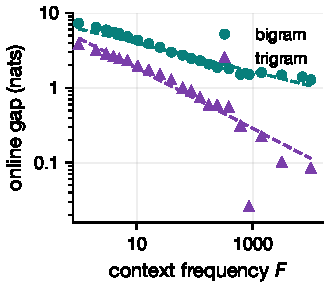
\includegraphics[width=\linewidth]{fig03a_frequency.pdf}
\subcaption{}
\label{fig:frequency}
\end{subfigure}\hfill
\begin{subfigure}{0.325\linewidth}
\centering
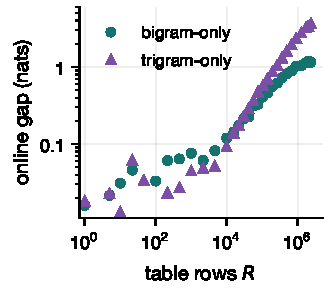
\includegraphics[width=\linewidth]{fig03b_capacity.pdf}
\subcaption{}
\label{fig:capacity}
\end{subfigure}\hfill
\begin{subfigure}{0.325\linewidth}
\centering
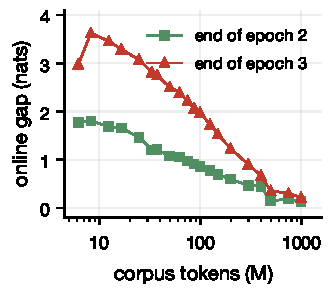
\includegraphics[width=\linewidth]{fig03c_corpus.pdf}
\subcaption{}
\label{fig:corpus-size}
\end{subfigure}
\caption{Empirical scaling laws of the gap: (a) context frequency, (b) table capacity, (c) training corpus size.}
\label{fig:scaling}
\end{figure}
\begin{figure}[!htbp]
\centering
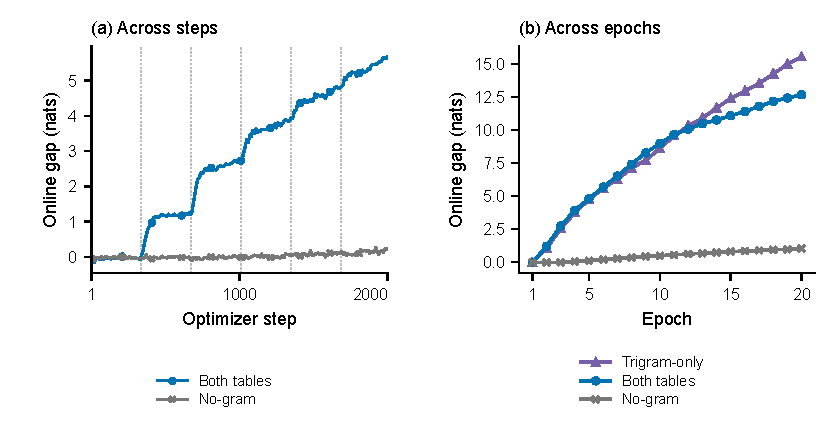
\includegraphics[width=0.9\linewidth]{fig06_replay.pdf}
\caption{Gap growth under replay: (a) within epochs, (b) across 20 epochs.}
\label{fig:staircase}
\end{figure}

\subsection{Causal interventions}
\label{sec:interventions}

Two interventions in the both-table model test the frequency account directly. Both use the fixed single-shard training corpus, run for 1000 updates, and start the intervention at step 338, after the first epoch; the two panels of Figure~\ref{fig:interventions} use independent runs, each with its own unmodified control.

\paragraph{Low-frequency retrieval masking.}
We count context frequencies in the unrepeated training corpus and mask the $n$-gram contribution whenever $F\leq\tau$, applying the rule separately to the bigram and trigram branches with thresholds $\tau\in\{1,2,4,8,200\}$. The retrieved embedding is set to zero during both training and evaluation, while the corresponding token remains in the training loss. Suppressing low-frequency memory access reduces the gap (Figure~\ref{fig:interventions}a): the excess gap is concentrated in rare contexts.

\paragraph{Freezing the tables.}
We train both $n$-gram tables normally during the first epoch, then freeze their parameters while continuing to update the backbone. A pronounced training--validation gap still develops after the tables are frozen (Figure~\ref{fig:interventions}b): once the tables hold learned context representations, the backbone alone can fit them during replay, so freezing the tables does not prevent forking.

\begin{figure}[!htbp]
\centering
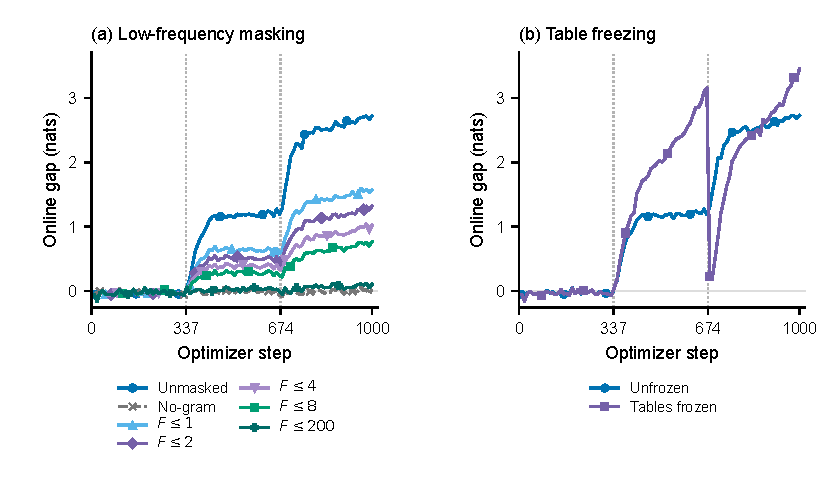
\includegraphics[width=0.88\linewidth]{fig07_interventions.pdf}
\caption{Causal interventions after epoch 1: (a) low-frequency retrieval masking, (b) table freezing.}
\label{fig:interventions}
\end{figure}
